\documentclass{beamer}
\usepackage{xmpmulti}
\usepackage[backend=biber]{biblatex}
\addbibresource{references.bib}

\title{Markowitz Portfolio Optimisation performance during COVID-19}
\author{Anna Stepuk, Arber Fetahu, Azizbek Asadov and Maxime Schweizer}
\date[14 December 2024]{University of Zurich
\newline
Digital Tools for Finance
\newline
\newline
14 December 2024}

\begin{document}

\begin{frame}
  \titlepage
\end{frame}

\begin{frame}{Summary}
\begin{itemize}
\item One of the recent market shocks that caused turmoil on the stock market was the COVID-19 pandemic (especially the first year)
\item By using blue-chip stocks data we constructed and optimized minimum variance and maximum Sharpe Ratio portfolios to test their performance in market distress 
\item As per our results, none of the suggested models could generate stable positive return, including equally weighted portfolio (which was used as a benchmark)
\item The maximum Sharpe Ratio portfolio lead to the highest Sharpe Ratio at the cost of risk, while the minimum Variance portfolio sacrificed returns for lower volatility
\end{itemize}
\end{frame}






\begin{frame}{Introduction}
The COVID-19 pandemic caused extreme volatility in financial markets globally.

\vspace{0.5cm}

The Modern Portfolio theory, based on the Mean-Variance analysis by Markowitz offers a tool:

\begin{itemize}
    \item To analyse risk and return in portfolios
    \item To construct optimal portfolios for a given level of risk
\end{itemize}

\vspace{0.5cm}

In this study, we analyze the application and performance of portfolios constructed according to Markowitz's proposal during the period of severe market turmoil caused by the COVID-19 pandemic

\end{frame}





\begin{frame}{Research Question}
What is the performance of the minimum variance portfolio (MVP) and the maximum Sharpe ratio portfolio (MSRP) of blue-chip securities compared to an equally weighted portfolio (benchmark) during the COVID-19 pandemic? 


\end{frame}




\begin{frame}{Data}

Time period analysed: 1 November 2019 until 1 November 2020

\vspace{0.5 cm}

Two datasets:

\begin{itemize}
    \item Daily adjusted closing prices of the 30 constituents of the Dow Jones Industrial Average
    \item 10-Year US Treasury yield, which served as the risk-free rate
\end{itemize}

\vspace{0.5cm}

Rebalancing is done by-weekly with a forecasting period of one month.

\end{frame}

\begin{frame}{Theoretical Framework}
\begin{itemize}
    \item Investors are risk-averse \cite{1lindquist2022advanced}
    \item With diversification, the unsystematic risk of a portfolio can be reduced if the assets are not perfectly correlated (confirmed by calculating correlation matrix) \cite{mangram2013simplified}
    \item The Efficient Frontier is comprised of all optimal portfolios that have the highest return for a given risk level \cite{mangram2013simplified}
    \item The \textbf{minimum variance portfolio (MVP)} is the optimal portfolio with the lowest possible risk (variance) for a given expected return (average daily return in October 2019) \cite{bodnar2024constructing}
    \item The \textbf{maximum Sharpe ratio portfolio (MSRP)} is the optimal portfolio that has highest ratio of excess return (difference between portfolio return and risk-free rate) to risk (volatility) \cite{bodnar2024constructing}

\end{itemize}

\end{frame}

\begin{frame}{Constraints and assumptions}
\begin{itemize}
    \item Short selling is not allowed 
    \item Weights sum up to 1
    \item Expected return is set at average daily return of given securities set in October 2019 
    \item No transaction costs or taxes
    \item Portfolio returns are normally distributed
    \item Log returns are used for both forecasting and back-testing purposes
    \item Portfolio performances were measure with: return, volatility and Sharpe ratio
\end{itemize}
\end{frame}

\begin{frame}{Implementation}
The implementation was done using Jupyter Notebook.

\vspace{0.5cm}

Based on the logarithmic returns of the DJIA constituents, the correlation matrix as well as the means, the variances, the skewnesses and the kurtoses were calculated.

\vspace{0.5cm}

We used the $cvxopt$-package (quadratic programming) to run the optimization problems with the given constrains.

\vspace{0.5cm}

We calculated performance measures for an equally-weighted portfolio, which we used as a benchmark.

\end{frame}


\begin{frame}{Results (Minimum Variance Portfolio, daily performance)}
    \begin{center}
        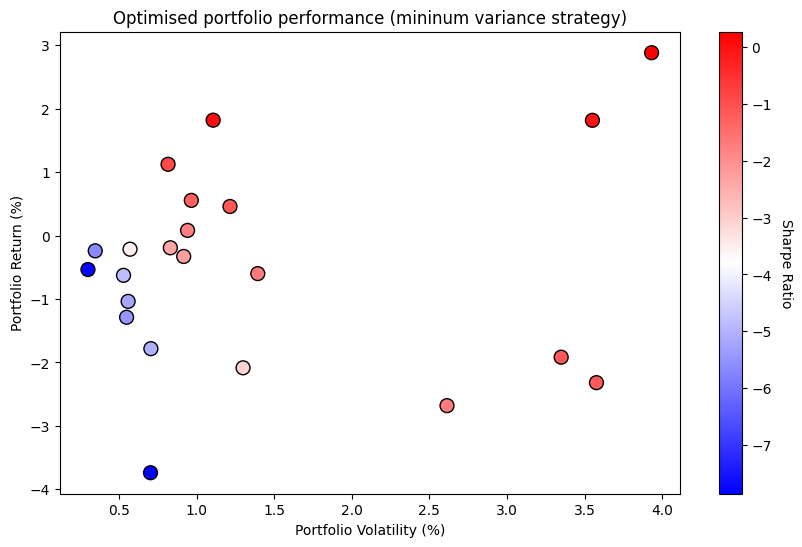
\includegraphics[width=0.8\textwidth]{resources/Optimised portfolio performance (minimum variance portfolio).png}
    \end{center}

As per obtained results, we observe that in the majority of cases, the Sharpe Ratio was negative (with negative returns), with the exception for few near zero (associated with higher volatility). 

\end{frame}


\begin{frame}{Results (Maximum Sharpe Ratio Portfolio, daily performance)}
    \begin{center}
        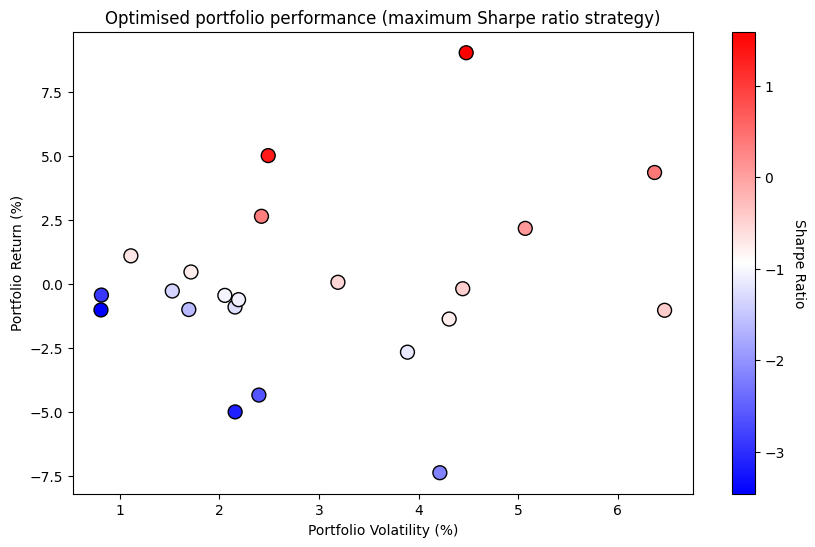
\includegraphics[width=0.8\textwidth]{resources/Optimised portfolio performance (maximum sharpe ratio strategy).png}
    \end{center}

As per obtained results, we observe more cases with positive Sharpe Ratio, however associated with higher volatility and return values.
\end{frame}

\begin{frame}{Results (Benchmark Portfolio, daily performance)}
    \begin{center}
        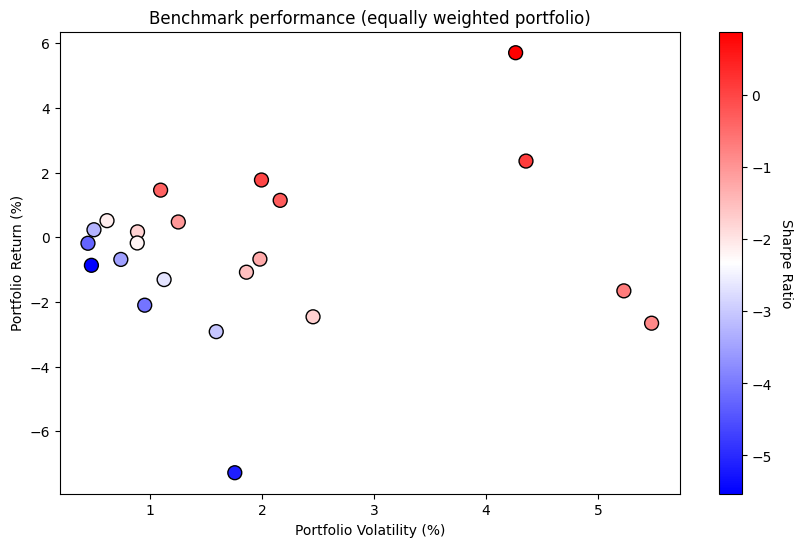
\includegraphics[width=0.8\textwidth]{resources/Benchmark performance (equally weighted portfolio).png}
    \end{center}
Performance of the equally weighted portfolio is more similar to MVP with few cases of positive Sharpe Ratio associated with higher volatility.  
\end{frame}

\begin{frame}{Results (Back-testing returns against benchmark, daily data)}
    \begin{center}
        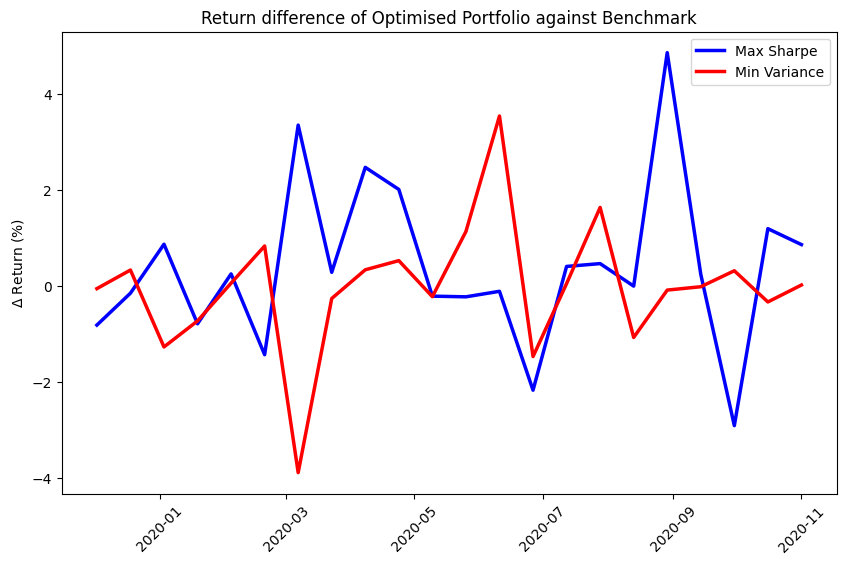
\includegraphics[width=0.7\textwidth]{resources/Return difference of Optimised Portfolio against Benchmark.png}
    \end{center}

\small {Based on the obtained results, the MSRP and MVP outperform the equally weighted portfolio only on a few instances. Interestingly, on the dates when the MSRP underperforms, the MVP delivers higher returns. }

\end{frame}

\begin{frame}{Results (Back-testing volatility against benchmark, daily data)}
    \begin{center}
        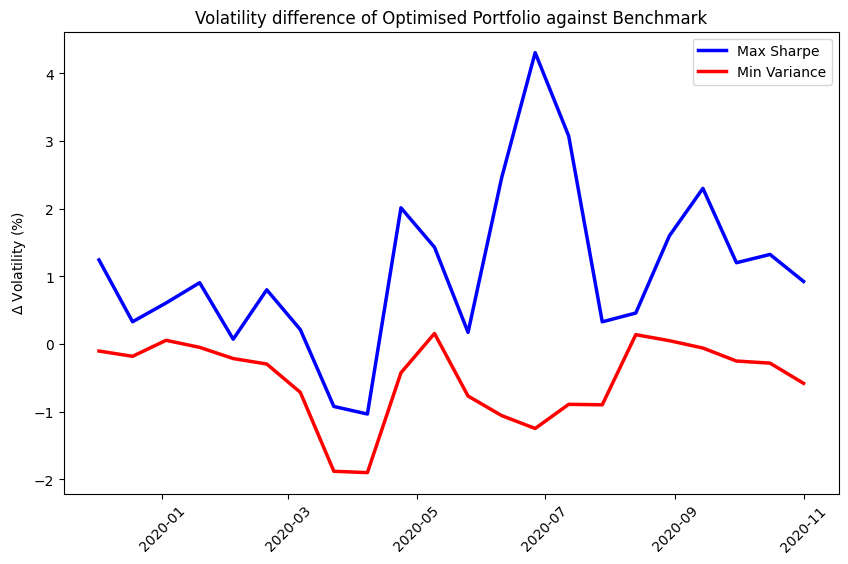
\includegraphics[width=0.7\textwidth]{resources/Volatility difference of Optimised Portfolio against Benchmark.png}
    \end{center}    
\small{Similarly to previously reported results, the MSRP has the highest volatility in comparison to other models. Interestingly, the MVP has the lowest volatility on average.}
\end{frame}

\begin{frame}{Results (Back-testing Sharpe Ratio against benchmark, daily data)}
    \begin{center}
        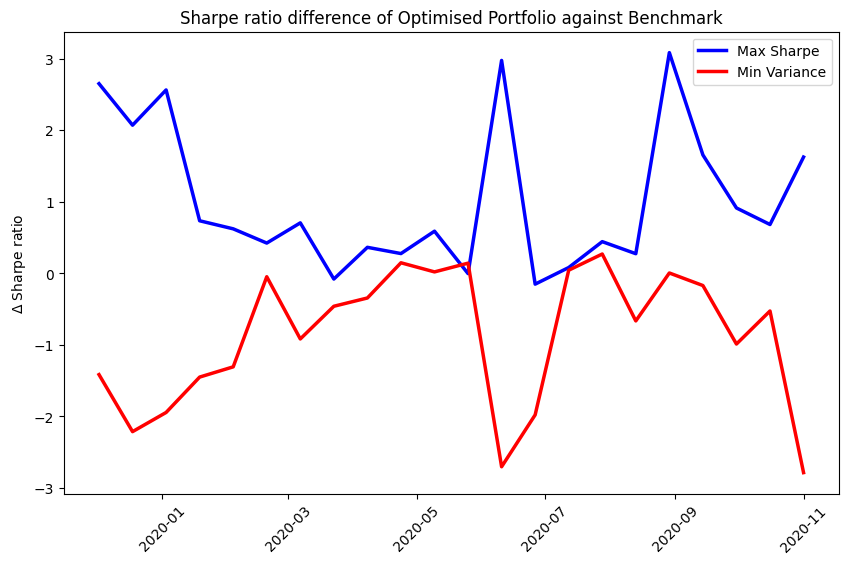
\includegraphics[width=0.7\textwidth]{resources/Sharpe ratio difference of Optimised Portfolio against Benchmark.png}
    \end{center}
\small{As expected, the MSRP delivers the highest Sharpe Ratio. The MVP, on the other side, underperformes in comparison to the other models.}
\end{frame}

\begin{frame}{Conclusion}
    \begin{itemize}
        \item In course of COVID-19 none of the models provided stable positive performance in terms of return, volatility and Sharpe ratio
        \item The MSRP generated more positive returns, however, at cost of higher risk (i.e. volatility)
        \item  The MVP, at the same time, resulted in the lowest volatility among the three models, however, often generating negative return
        \item Overall, beating the benchmark (equally weighted portfolio) performance proved to be difficult during the market distress situation
        \item At the same time, it's important to assess the performance of other hedging instruments (such as commodity futures, TIPS etc.) to construct more optimal and diversified portfolio
    \end{itemize}
\end{frame}

\begin{frame}{References}
\printbibliography
\end{frame}

\end{document}
